\documentclass[12pt]{beamer}
\usepackage{../Estilos/BeamerMAF}
\usetheme{Dresden}
\usecolortheme{seahorse}
%\useoutertheme{default}
\setbeamercovered{invisible}
% or whatever (possibly just delete it)
\setbeamertemplate{section in toc}[sections numbered]
\setbeamertemplate{subsection in toc}[subsections numbered]
\setbeamertemplate{subsection in toc}{\leavevmode\leftskip=3.2em\rlap{\hskip-2em\inserttocsectionnumber.\inserttocsubsectionnumber}\inserttocsubsection\par}
\setbeamercolor{section in toc}{fg=blue}
\setbeamercolor{subsection in toc}{fg=blue}
\setbeamercolor{frametitle}{fg=blue}
\setbeamertemplate{caption}[numbered]

\setbeamertemplate{footline}
\beamertemplatenavigationsymbolsempty
\setbeamertemplate{headline}{}

\makeatletter
\setbeamercolor{section in foot}{bg=gray!30, fg=black!90!orange}
\setbeamercolor{subsection in foot}{bg=blue!30!yellow, fg=red}
\setbeamertemplate{footline}
{
  \leavevmode%
  \hbox{%
  \begin{beamercolorbox}[wd=.333333\paperwidth,ht=2.25ex,dp=1ex,center]{section in foot}%
    \usebeamerfont{section in foot} \insertsection
  \end{beamercolorbox}}%
  \begin{beamercolorbox}[wd=.333333\paperwidth,ht=2.25ex,dp=1ex,center]{subsection in foot}%
    \usebeamerfont{subsection in foot}  \insertsubsection
  \end{beamercolorbox}%
  \begin{beamercolorbox}[wd=.333333\paperwidth,ht=2.25ex,dp=1ex,right]{date in head/foot}%
    \usebeamerfont{date in head/foot} \insertshortdate{} \hspace*{2em}
    \insertframenumber{} / \inserttotalframenumber \hspace*{2ex} 
  \end{beamercolorbox}}%
  \vskip0pt%
\makeatother 

\makeatletter
\patchcmd{\beamer@sectionintoc}{\vskip1.5em}{\vskip0.8em}{}{}
\makeatother


\date{29 de octubre de 2021}

\title{\large{Funciones y valores propios}}
\subtitle{Tema 3 - Bases completas y ortogonales}
\author{M. en C. Gustavo Contreras Mayén}

\begin{document}
\maketitle
\fontsize{14}{14}\selectfont
\spanishdecimal{.}

\section*{Contenido}
\frame{\tableofcontents[currentsection, hideallsubsections]}

\section{Ecuaciones diferenciales tipo S-L}
\frame{\tableofcontents[currentsection, hideothersubsections]}
\subsection{Ecuaciones de la física matemática}

\begin{frame}
\frametitle{Ecuaciones relevantes}
Veremos algunas de las EDO que son importantes en la física matemática, y su forma autoadjunta.
\\
\bigskip
\pause
Las soluciones se conocen como \textcolor{blue}{funciones especiales}, ya que no se expresan en términos de funciones elementales.
\end{frame}
\begin{frame}
\frametitle{Ecuación asociada de Legendre}
\begin{align*}
(1 -x^{2}) \, \sderivada{y} - 2 \, x \, \pderivada{y} + \bigg[ \ell (\ell + 1) - \dfrac{m^{2}}{1 - x^{2}} \bigg] \, y = 0
\end{align*}
\pause
Forma autoadjunta:
\begin{align*}
\dv{x} \bigg[ (1 - x^{2}) \, \pderivada{y} \bigg] \bigg[ \ell (\ell + 1) - \dfrac{m^{2}}{1 - x^{2}} \bigg] \, y = 0
\end{align*}
\pause
Soluciones: Polinomios asociados de Legendre $L_{n}^{k} (x)$.
\end{frame}
\begin{frame}
\frametitle{Ecuación ordinaria de Legendre}
\begin{align*}
(1 -x^{2}) \, \sderivada{y} - 2 \, x \, \pderivada{y} + \ell (\ell + 1) \, y = 0
\end{align*}
\pause
Forma autoadjunta:
\begin{align*}
\dv{x} \bigg[ (1 - x^{2}) \, \pderivada{y} \bigg] + \ell (\ell + 1) \, y = 0
\end{align*}
\pause
Soluciones: Polinomios ordinarios de Legendre $L_{n}(x)$.
\end{frame}
\begin{frame}
\frametitle{Ecuación confluente hipergeométrica}
\begin{align*}
x \, \sderivada{y} + (c - x) \, \pderivada{y} - a \, y = 0
\end{align*}
\pause
Forma autoadjunta:
\begin{align*}
\dv{x} \bigg[ x^{c} \, e^{-x} \, \pderivada{y} \bigg] - a \, x^{c-1} \, e^{-x} \, y = 0
\end{align*}
\pause
Soluciones: Funciones hipergeométricas confluentes $M(a ;c ;x)$. Donde $a, c \in \mathbb{R}, c \neq 0, -1, -2, \ldots$ y $x > 0$.
\end{frame}
\begin{frame}
\frametitle{La ecuación hipergeométrica}
Las ecuaciones hipergeométricas se presentan en una variedad de aplicaciones como:
\setbeamercolor{item projected}{bg=blue!70!black,fg=yellow}
\setbeamertemplate{enumerate items}[circle]
\begin{enumerate}[<+->]
\item Estadística.
\item Investigación de operaciones.
\item Mecánica cuántica.
\item Ecuaciones funcionales.
\item Vibración de placas.
\item Etc.
\end{enumerate}
\end{frame}
\begin{frame}
\frametitle{Ecuación ordinaria de Bessel}
\begin{align*}
x^{2} \, \sderivada{y} + x \, \pderivada{y} + ( k^{2} \, x^{2} - \nu^{2}) \, y = 0
\end{align*}
\pause
Forma autoadjunta:
\begin{align*}
\dv{x} \big[ x \, \pderivada{y} \big] + \bigg[ k^{2} \, x - \dfrac{\nu}{x} \bigg] \, y = 0
\end{align*}
\pause
Soluciones: Funciones de Bessel $J_{n}(x)$.
\end{frame}
\begin{frame}
\frametitle{Otras ecuaciones de la física matemática}
Encontraremos otras EDO que nos conducirán a un conjunto que extiende a las funciones especiales.
\\
\bigskip
\pause
Que se revisarán tanto en el Tema 4, como en el Tema 5 del curso.
\end{frame}
\begin{frame}
\frametitle{Más ecuaciones de la física matemática}
\setbeamercolor{item projected}{bg=blue!70!black,fg=yellow}
\setbeamertemplate{enumerate items}[circle]
\begin{enumerate}[<+->]
\item Hipergeométrica ordinaria: \\
$x (x - 1) \, \sderivada{y} + \bigg[ (1 + a + b) \, x - c \bigg] \, \pderivada{y} + a \, b \, y = 0$
\item Chebyshev Tipo I: \\
$(1 - x^{2}) \, \sderivada{y} - x \, \pderivada{y} + n^{2} \, y = 0$
\item Chebyshev Tipo II: \\
$(1 - x^{2}) \, \sderivada{y} - 3 x \, \pderivada{y} + n(n + 2) \, y = 0$
\item Laguerre ordinaria: \\
$x \, \sderivada{y} + (1 - x) \, \pderivada{y} + n \, y = 0$
\seti
\end{enumerate}
\end{frame}
\begin{frame}
\frametitle{Más ecuaciones de la física matemática}
\setbeamercolor{item projected}{bg=blue!70!black,fg=yellow}
\setbeamertemplate{enumerate items}[circle]
\begin{enumerate}[<+->]
\conti    
\item Laguerre asociada: \\
$x \, \sderivada{y} + (k + 1 - x) \, \pderivada{y} + n \, y = 0$
\item Hermite: \\
$\sderivada{y} - 2 \, x \, \pderivada{y} + 2 \, \alpha \, y = 0$
\item Gegenbauer: \\
$(1 - x^{2}) \, \sderivada{y} - 2 (1 + \beta) \, x \, \pderivada{y} + n(n + 2 \, \beta + 1) \, y = 0$
\end{enumerate}
\end{frame}

\section{Problema de valores propios}
\frame{\tableofcontents[currentsection, hideothersubsections]}
\subsection{Problema tipo Sturm-Liouville}

\begin{frame}
\frametitle{Enunciado del ejercicio}
Resuelve el problema de tipo Sturm-Liouville:
\pause
\begin{align*}
x^{2} \, \sderivada{y} + 5 \, x \, \pderivada{y} + \lambda \, y = 0
\end{align*}
con las condiciones:
\begin{align*}
y(1) = y(e) = 0 \hspace{1.5cm} 1 \leq x \leq e
\end{align*}
\pause
Resolver el ejercicio implica obtener los correspondientes valores propios, funciones propias y revisar la ortogonalidad de éstas.
\end{frame}
\begin{frame}
\frametitle{La EDO}
Tomemos en cuenta que la forma de esta ecuación es:
\pause
\begin{align*}
a_{2} (x) \, \sderivada{y} + a_{1} (x) \, \pderivada{y} + a_{0}(x) \, y + \lambda \, y = f(x)
\end{align*}
\pause
se tiene que:
\begin{align*}
a_{2} = x^{2}, \hspace{0.5cm} a_{1} = 5\, x, \hspace{0.5cm} a_{0} = 0
\end{align*}
\end{frame}
\begin{frame}
\frametitle{Forma de tipo Sturm-Liouville}
Recordemos que la forma de tipo Sturm-Liouville es:
\pause
\begin{align*}
\dv{x} \left( p(x) \, \dv{x} \right) + q(x) \, y + \lambda \, \sigma (x) \, y = 0
\end{align*}
donde:
\begin{align*}
p(x) &= \dfrac{1}{a_{2}(x)} \, \exp \left( \scaleint{5ex} \, \dfrac{a_{1}(x)}{a_{2}(x)} \dd{x} \right) \\[0.5em]
q(x) &= p(x) \, \dfrac{a_{0}(x)}{a_{2}(x)} \\[0.5em]
F(x) &= p(x) \, \dfrac{f(x)}{a_{2}(x)}
\end{align*}
\end{frame}
\begin{frame}
\frametitle{Buscando la forma autoadjunta}
Entonces:
\pause
\begin{eqnarray*}
\begin{aligned}
p(x) &= \dfrac{1}{a_{2}(x)} \exp \left( \scaleint{5ex} \dfrac{a_{1}(x)}{a_{2}(x)} \dd{x} \right) = \\[0.5em] \pause
&= \dfrac{1}{x^{2}} \, \exp \left( \scaleint{5ex} \dfrac{5 x}{x^{2}} \dd{x} \right) = \\[0.5em] \pause
&= \dfrac{1}{x^{2}} \,  \exp \left( 5 \, \scaleint{5ex} \, \dfrac{1}{x} \dd{x} \right) = \\[0.5em] \pause
&= \dfrac{1}{x^{2}} \,  \exp \left( 5 \, \ln x \right) = \pause x^{3} > 0
\end{aligned}
\end{eqnarray*}
\end{frame}
\begin{frame}
\frametitle{Las funciones $q(x)$ y $F(x)$}
Se tiene además que:
\pause
\begin{align*}
q(x) = 0 \hspace{1.5cm} F(x) = 0
\end{align*}
\pause
Por lo que la EDO en forma de tipo Sturm-Liouville es:
\pause
\begin{align*}
\dv{x} \big( x^{5} \, \pderivada{y} \big) + \lambda \, x^{3} \, y = 0
\end{align*}
\end{frame}
\begin{frame}
\frametitle{Suposición en el problema}
Haremos la suposición que el problema es de tipo autoadjunto (Hermitiano), ya que con este primer material solo se revisará el cambio a problema de tipo Sturm-Liouville y obtener los valores propios y funciones propias.
\\
\bigskip
\pause
Con el material de la siguiente semana: operadores autoadjuntos, se comprobará efectivamente que el problema es Hermitiano.
\end{frame}
\begin{frame}
\frametitle{Consecuencia de ser autoadjunto}
Al cumplirse que es un problema autoadjunto, se tiene que los valores propios son reales y las funciones propias son ortogonales.
\end{frame}
\begin{frame}
\frametitle{Ecuación a resolver}
La ecuación que debemos de resolver es:
\begin{align*}
x^{2} \, \sderivada{y} + 5 \, x \, \pderivada{y} + \lambda \, y = 0
\end{align*}
\pause
Identificamos que es una ecuación de tipo Euler, con $y(x) = x^{m}$
\end{frame}
\begin{frame}
\frametitle{Ecuación característica}
La ecuación característica es:
\pause
\begin{align*}
m^{2} + 4 \, m + \lambda = 0
\end{align*}
\pause
entonces:
\begin{align*}
m = - 2 \pm \sqrt{4 - \lambda}
\end{align*}
\end{frame}
\begin{frame}
\frametitle{Solución general}
La solución general de la EDO es:
\pause
\begin{align*}
y(x) = \dfrac{1}{x^{2}} \, \left( a \, x^{\sqrt{4 - \lambda}} + b \, x^{- \sqrt{4 - \lambda}} \right)
\end{align*}
\end{frame}
\begin{frame}
\frametitle{Las CDF}
De las CDF, se tiene que $y(1) = 0$, \pause entonces $b = -a$, así:
\pause
\begin{align*}
y(x) = \dfrac{a}{x^{2}} \, \left( x^{\sqrt{4 - \lambda}} + x^{- \sqrt{4 - \lambda}} \right)
\end{align*}
\end{frame}
\begin{frame}
\frametitle{La segunda CDF}
Con la condición $y(e) = 0$, se llega a:
\pause
\begin{itemize}
\item Si $4 - \lambda > 0$
\pause
\begin{eqnarray*}
\Rightarrow \hspace{0.3cm} \sinh \sqrt{4 - \lambda} = 0 \\[0.5em] \pause 
\lambda = 4
\end{eqnarray*}
\pause
Por tanto $y(x) = 0$
\end{itemize}
\end{frame}
\begin{frame}
\frametitle{La segunda CDF}
Con la condición $y(e) = 0$, se llega a:
\pause
\begin{itemize}
\item Si $4 - \lambda < 0$
\pause
\begin{eqnarray*}
\Rightarrow \hspace{0.3cm} \sen \sqrt{4 - \lambda} &=& 0 \\[0.5em] \pause 
\sqrt{\lambda - 4} &=& n \, \pi \\[0.5em] \pause
\lambda &=& 4 + n^{2} \, \pi^{2}
\end{eqnarray*}
\end{itemize}
\end{frame}
\begin{frame}
\frametitle{La solución general}
La solución general se expresa como:
\begin{align*}
y(x) &= \dfrac{a}{x^{2}} \left( x^{i n \pi} - x^{-i n \pi} \right)
\end{align*}
\pause
como $x = e^{\ln x}$, tendremos que:
\pause
\begin{eqnarray*}
y(x) &=& \dfrac{a}{x^{2}} \bigg[ \exp \big( i \, n \, \pi \, \ln x \big) -  \exp \big( - i \, n \, \pi \, \ln x \big) \bigg] = \\[0.5em] \pause
&=& \dfrac{a}{x^{2}} \, 2 \, i \, \sin (n \, \pi \, \ln x)
\end{eqnarray*}
\end{frame}
\begin{frame}
\frametitle{Valores propios y funciones propias}
El conjunto de valores propios es:
\pause
\begin{align*}
\left\{ \lambda_{n} \right\} = 4 + n^{2} \, \pi^{2}
\end{align*}
\def\arraystretch{1}
\begin{tabular}{c c}
$\lambda_{1} =$ & $13.8696$ \\
$\lambda_{2} =$ & $43.4784$ \\
$\lambda_{3} =$ & $92.8264$ \\
$\lambda_{4} =$ & $161.914$ \\
$\vdots$
\end{tabular}
\end{frame}
\begin{frame}
\frametitle{Valores propios y funciones propias}
El conjunto de las funciones propias es:
\pause
\begin{align*}
\left\{ y_{n} (x) \right\} = \left\{ \dfrac{1}{x^{2}} \sin (n \, \pi \, \ln x) \right\}
\end{align*}
Tomemos en cuenta que las funciones aún no están normalizadas.
\end{frame}
\begin{frame}
\frametitle{La ortogonalidad de las funciones}
Revisando la ortogonalidad:
\pause
\begin{eqnarray*}
\begin{aligned}
&\scaleint{5ex}_{\bs x=1}^{x=e} \, p(x) \, y_{n}^{*} (x) \, y_{m}(x) \dd{x} = \\[0.5em] \pause
&= \scaleint{5ex}_{\bs x=1}^{x=e} \, \sin (n \, \pi  \, \ln x) \, \sin (m \, \pi  \, \ln x) \dd{x}
\end{aligned}
\end{eqnarray*}
\pause
\end{frame}
\begin{frame}
\frametitle{Resolviendo la integral}
Como $x = e^{u}$, entonces:
\begin{align*}
\scaleint{5ex}_{\bs 0}^{1} \, \sin (n \, \pi  \, u) \, \sin (m \, \pi  \, u) \dd{u} = 0 \hspace{1cm} m \neq n
\end{align*}
\pause
Si $m = n$, se tiene que:
\begin{align*}
\scaleint{5ex}_{\bs x=1}^{x=e} \, p(x) \, y_{n}^{2} (x) \dd{x} = \dfrac{\pi}{2}
\end{align*}
\end{frame}
\begin{frame}
\frametitle{Funciones propias normalizadas}
El conjunto de funciones propias normalizadas, con la función de peso $p(x) = x^{3}$ en el intervalo $1 \leq x \leq e$ es:
\begin{align*}
\left\{ y_{n} (x) \right\} = \left\{ \sqrt{\dfrac{2}{\pi}} \, \dfrac{\sin (n \, \pi \, \ln x)}{x^{2}} \right\}
\end{align*}
\end{frame}
\begin{frame}
\frametitle{Gráfica de las funciones propias}
\begin{figure}
    \centering
    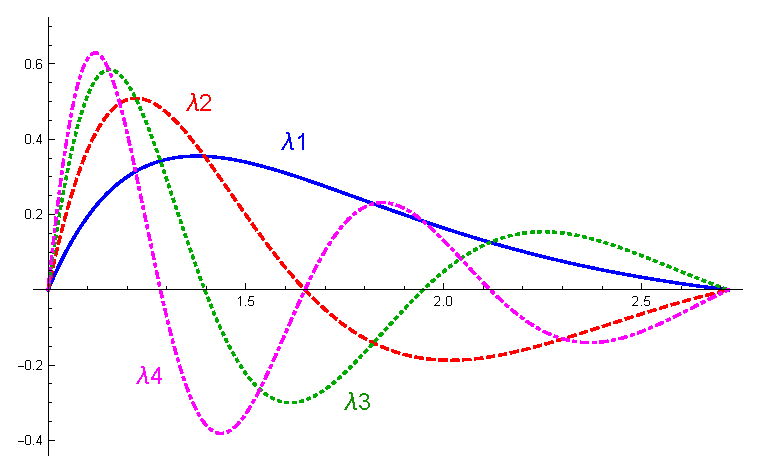
\includegraphics[scale=0.85]{Imagenes/Ejercicio_SL_01_Funciones.eps}
\end{figure}
\end{frame}

\subsection{Segundo ejercicio}

\begin{frame}
\frametitle{Siguiente ejericio}
Calcula los valores propios y las funciones propias de la siguiente EDO definida en $0 \leq x \leq a$:
\pause
\begin{align*}
\dv[2]{\psi}{x} + \lambda \, \psi = 0   
\end{align*}
con las siguientes condiciones:
\begin{align*}
\psi_{x}(0) = 0 \hspace{1.5cm} \psi_{x}(a) - \dfrac{\psi(a)}{a} = 0
\end{align*}
\end{frame}
\begin{frame}
\frametitle{Revisando el valor de $\lambda$}
\textbf{1.} Si $\lambda < 0$, podemos escribir la EDO como:
\pause
\begin{align*}
\dv[2]{\psi}{x} - \lambda \, \psi = 0   
\end{align*}
\pause
Cuya solución es:
\begin{align*}
\psi(x) = A \, e^{k x} + B \, e^{-k x}
\end{align*}
\end{frame}
\begin{frame}
\frametitle{Revisando las CDF}
Con la condición $\psi_{x}(0) = 0$, se tiene que:
\pause
\begin{align*}
B = - A
\end{align*}
\pause
Por lo tanto:
\pause
\begin{align*}
\psi(x) = A \, \cosh (k x)
\end{align*}
\end{frame}
\begin{frame}
\frametitle{Segunda condición}
De la segunda condición:
\begin{align*}
\psi_{x}(a) - \dfrac{\psi(a)}{a} = 0
\end{align*}
\pause
Se tiene que:
\pause
\begin{align*}
(k \, a) \, \tanh(k \, a) = 1
\end{align*}
siendo una expresión trascendental, cuya solución devuelve el único valor:
\begin{align*}
k \, a = 1.2
\end{align*}
\end{frame}
\begin{frame}
\frametitle{Valor propio obtenido}
Por lo tanto:
\begin{eqnarray*}
\lambda_{0} = - k^{2} = \pause - \dfrac{1.44}{a^{2}}
\end{eqnarray*}
\pause
por lo que la solución es:
\pause
\begin{align*}
\psi (x) \varpropto \cosh \left( \dfrac{1.2 \, x}{a} \right)
\end{align*}
\pause
La función propia no tiene ceros en $(0, a)$ y es única: \emph{un valor propio, una función propia}.
\end{frame}
\begin{frame}
\frametitle{Gráfica de la única función propia, $a = 4$}
\begin{figure}
    \centering
    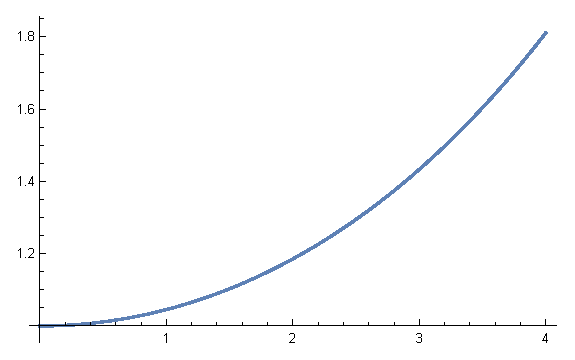
\includegraphics[scale=1]{Imagenes/Ejercicio_SL_02_Funciones.eps}
\end{figure}
\end{frame}
\begin{frame}
\frametitle{Siguiente caso}
\textbf{2.} Si $\lambda > 0$, escribimos la EDO como:
\pause
\begin{align*}
\dv[2]{\psi}{x} + k^{2} \, \psi = 0   
\end{align*}
\pause
cuya solución es:
\pause
\begin{align*}
\psi(x) = A \, \exp(i \, k \, x) +  B \, \exp (- i \, k \, x)
\end{align*}
\end{frame}
\begin{frame}
\frametitle{Ocupando las CDF}
Al utilizar las CDF, se llega a:
\pause
\begin{align*}
(k \, a) \, \tan (k \, a) = -1
\end{align*}
\pause
que tiene una secuencia infinita de raíces.
\\
\bigskip
\pause
Se tiene un \emph{espectro infinito y discreto de valores propios y funciones propias.}
\end{frame}
\begin{frame}
\frametitle{Entrega de actividades}
La entrega de las actividades programadas para este día: 29 de octubre:
\\
\bigskip
\pause
Se extiende el plazo para el domingo 31 de octubre a las 20 pm.
\end{frame}
\begin{frame}
\frametitle{Entrega de actividades}
Para mantener la consideración en los plazos de las entregas, se requiere que al menos el $75\%$ de las alumnas y alumnos que han enviado sus actividades, mantenga la entrega. En caso contrario, se deberán de enviar las actividades como se acordó desde el inicio del semestre.
\end{frame}
\end{document}